\chapter{Máscara}


\section{Operações booleanas}

Após efetuar segmentações, é possível realizar operações booleanas entre as máscaras. As operações booleanas suportadas são:\\
\\
\textbf{União}, realiza a união de duas máscaras;\\
\textbf{Diferença}, realiza a diferença entre a primeira máscara com a segunda;\\
\textbf{Intersecção}, para apagar marcadores de objeto ou fundo.\\
\textbf{Disjunção exclusiva}, também é conhecida como XOR, mantém as regiões de ambas as máscara que possuem diferença.\\

Para ativar essa ferramenta é necessário ir no menu \textbf{Ferramentas}, \textbf{Operações boolenas}, como é exibido na figura~\ref{fig:booleano_menu} 

\begin{figure}[!htb]
\centering
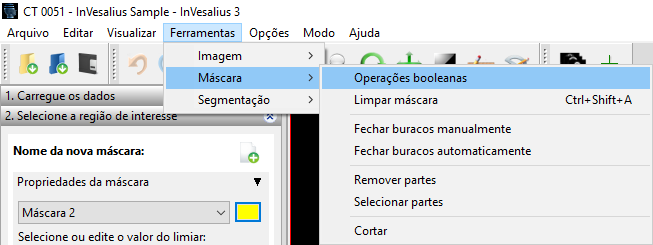
\includegraphics[scale=0.5]{mask_operation_boolean_menu_pt.png}
\caption{Menu para ativar a ferramenta de operações booleanas.}
\label{fig:booleano_menu}
\end{figure}

É necessário selecionar a primeira máscara, a operação a ser realizada e a segunda máscara conforme mostra a figura~\ref{fig:booleano_janela}. Em seguida é necessário clicar no botão \textbf{Ok}.

\begin{figure}[!htb]
\centering
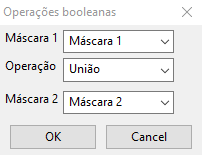
\includegraphics[scale=0.5]{mask_boolean_dialog_pt.png}
\caption{Ferramenta de operações booleanas.}
\label{fig:booleano_janela}
\end{figure}

Na figura~\ref{fig:op_boolana}, apresentamos um exemplo de utilização da ferramenta.

\begin{figure}[!htb]
  \centering
  \subfloat[Máscara A]{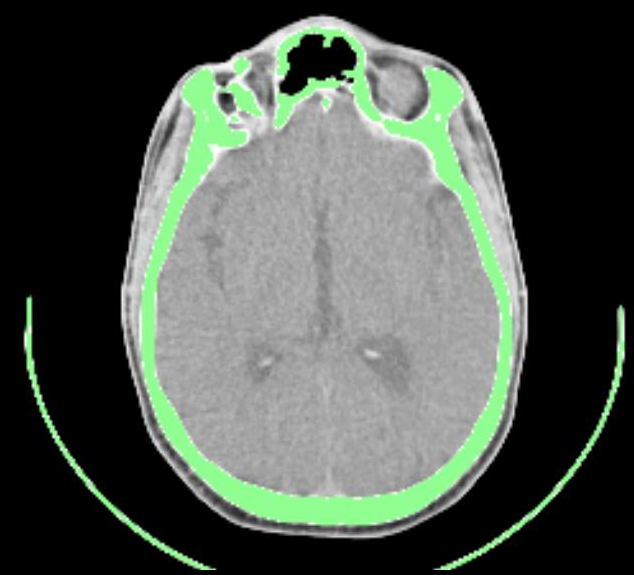
\includegraphics[width=0.332\textwidth]{booleano_m_a.png}}                
  \hfill
  \subfloat[Máscara B]{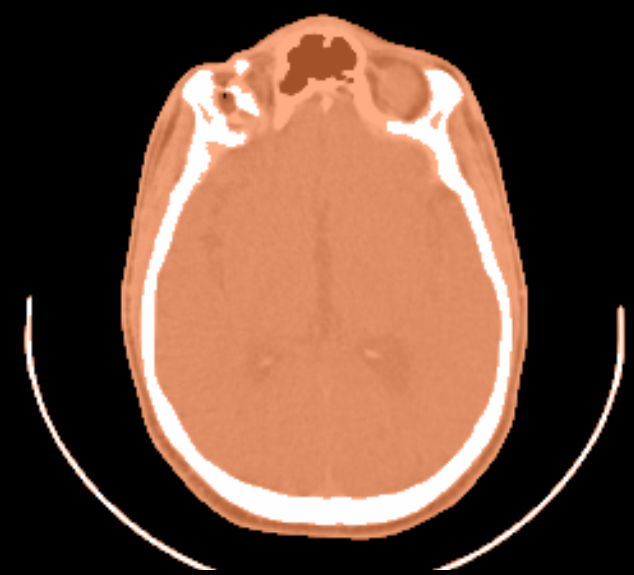
\includegraphics[width=0.332\textwidth]{booleano_m_b.png}}	
  \hfill  
  \subfloat[União (A $\cup$ B)]{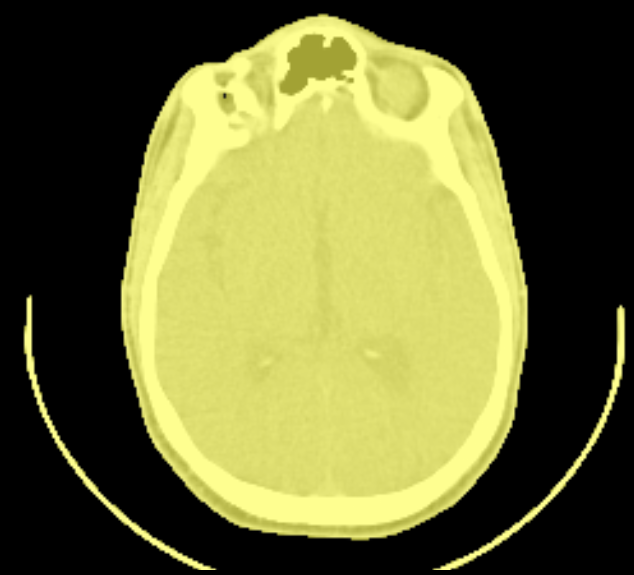
\includegraphics[width=0.332\textwidth]{booleano_uniao.png}}
  \hfill  
  \subfloat[Diferença (A - B)]{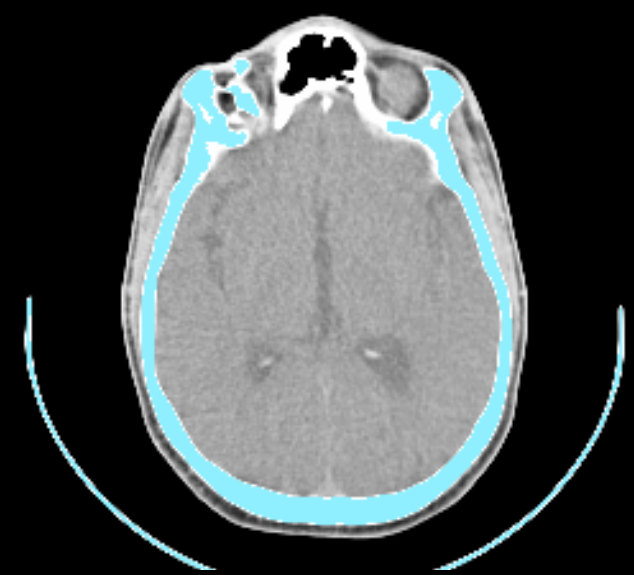
\includegraphics[width=0.332\textwidth]{booleano_dif.png}}
  \hfill  
  \subfloat[Intersecção (A $\cap$ B)]{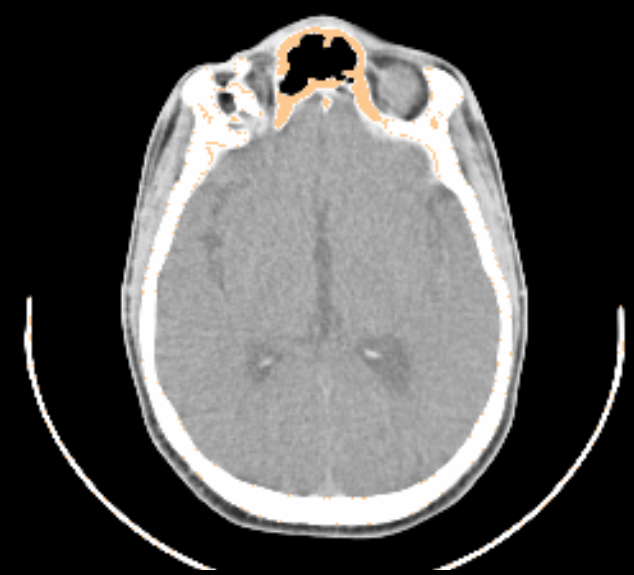
\includegraphics[width=0.332\textwidth]{booleano_interc.png}}
  \hfill  
  \subfloat[Disjunção exclusiva (A $\oplus$ B)]{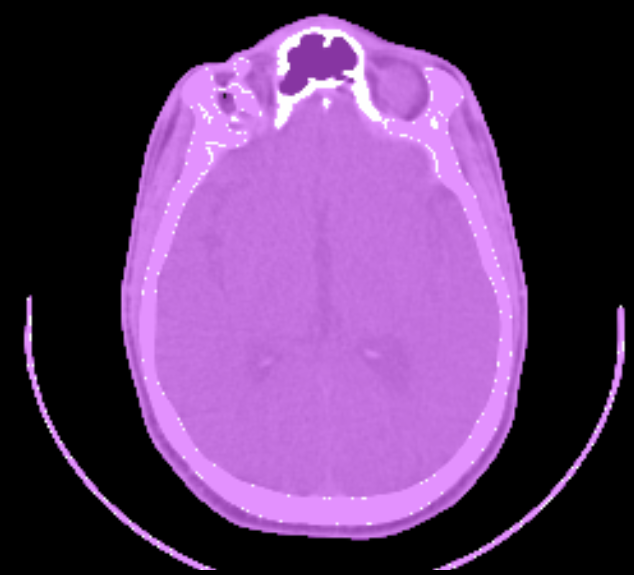
\includegraphics[width=0.332\textwidth]{booleano_disj_exc.png}}
  \caption{Exemplo de operações booleanas.}
  \label{fig:op_boolana}
\end{figure}

\section{Limpeza total da máscara}
\label{cap:limpeza_mascara}

Pode-se efetuar a limpeza total da máscara (figura~\ref{fig:limpeza_mascara}), isso é recomendado antes de iniciar a inserção de marcadores de Watershed. A ferramenta está localizada no menu, \textbf{Ferramentas}, \textbf{Máscara}, \textbf{Limpar máscara}, também é possível executa-la pressionando as teclas \textbf{CTRL+SHIFT+A}.

\begin{figure}[!htb]
\centering
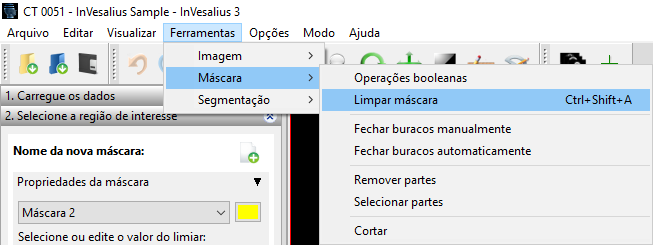
\includegraphics[scale=0.5]{mask_clean_menu_pt.png}
\caption{Limpeza de máscara}
\label{fig:limpeza_mascara}
\end{figure}

\section{Fechar buracos manualmente}

Ao realizar a segmentação é possível que pequenas partes (buracos) que deseja-se ser selecionadas não sejam e ao gerar a superfície para a impressão 3D pode ser que ocorra inconsistências por causa desses buracos, para evitar esse tipo de problema é recomendável preenche-los. Para isso é basta acessar o menu \textbf{Ferramentas}, \textbf{Máscara} e por último clicar em \textbf{Fechar buracos manualmente} (figura~\ref{fig:menu_mask_manual_fill_holes}). Em seguida será exibido uma tela (figura~\ref{fig:mask_manual_fill_holes_window}) para configurar os parâmetros.

\begin{figure}[!htb]
\centering
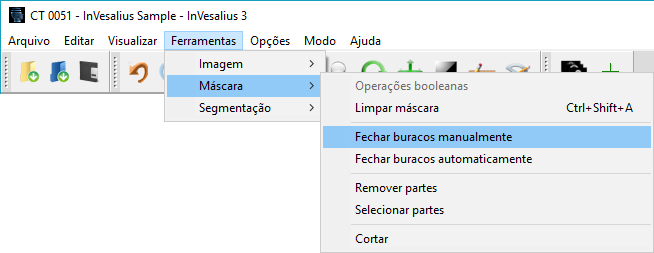
\includegraphics[scale=0.4]{menu_mask_manual_fill_holes_pt.png}
\caption{Menu para acessa a ferramenta de fechamento de buracos manual.}
\label{fig:menu_mask_manual_fill_holes}
\end{figure}

\begin{figure}[!htb]
\centering
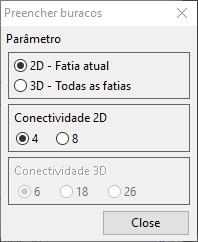
\includegraphics[scale=0.7]{mask_manual_fill_holes_window_pt.png}
\caption{Tela para configurar parâmetros de fechamento de buracos.}
\label{fig:mask_manual_fill_holes_window}
\end{figure}

Entre os parâmetros existe a opção de realizar o fechamento de buraco levando em consideração somente a fatia atual (\textbf{2D - Fatia Atual}) ou todas as fatias (\textbf{3D - Todas as fatias}) e suas respectivas conectividades, no caso 2D, conectividade $4$ ou $8$, conectividade $6$,$18$ ou $26$. No caso 3D se houver conectividade no buraco em diferentes fatias ele irá expandir para as demais fatias.

Quando os parâmetros estiverem configurados, clique com o \textbf{botão esquerdo} do mouse sobre o buraco que deseja-se fechar.

Podemos observar na imagem~\ref{fig:mask_fill_hole}.a, um exemplo de uma máscara sem preenchimento de buracos e outra com os buracos preenchidos (imagem~\ref{fig:mask_fill_hole}.b). Após o uso da ferramenta, para sair clique no botão \textbf{fechar ou close} no canto inferior direito da janela de configuração de parâmetros.

\begin{figure}[!htb]
  \centering
  \subfloat[Buracos]{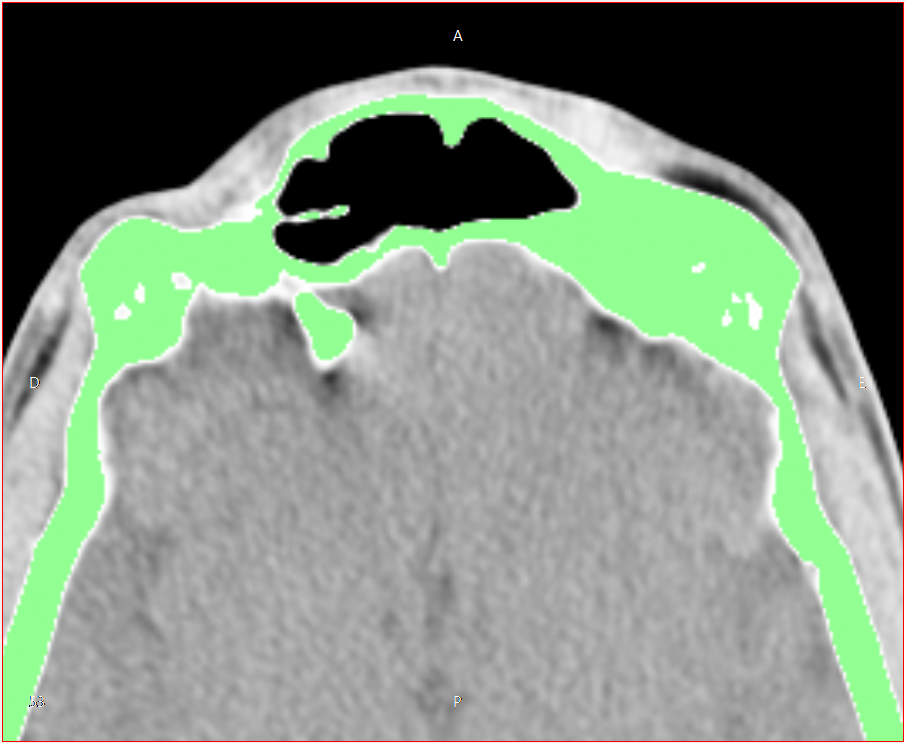
\includegraphics[width=0.4\textwidth]{mask_axial_with_hole.png}}  \qquad
  \subfloat[Buracos fechados]{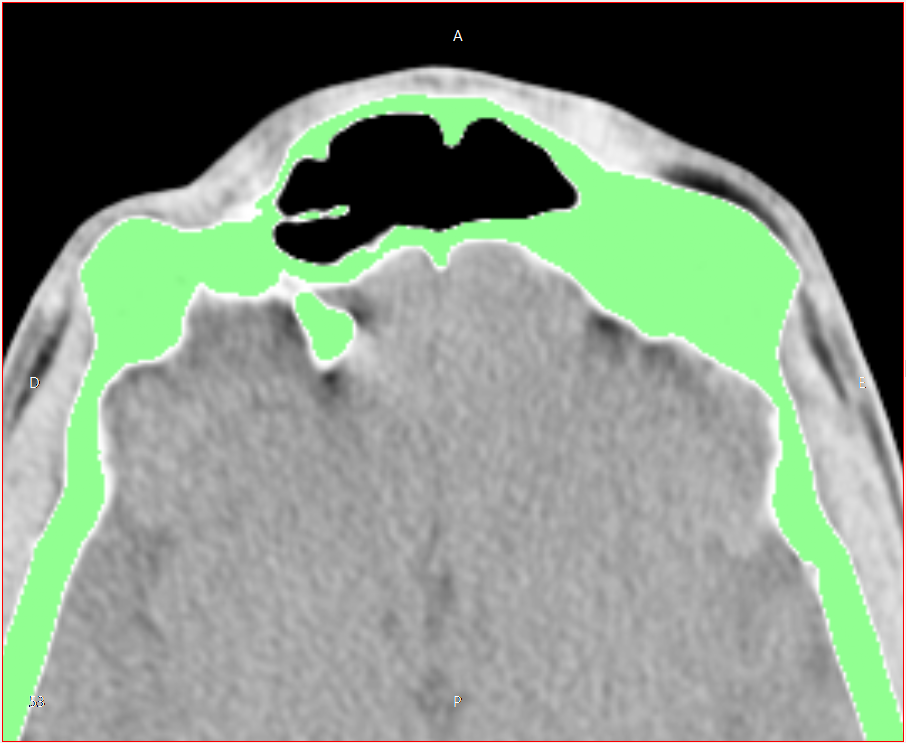
\includegraphics[width=0.4\textwidth]{mask_axial_filled_hole.png}}
  \hfill
  \caption{Exemplo de máscara com buracos e buracos preenchidos.}
  \label{fig:mask_fill_hole}
\end{figure}


\section{Fechar buracos automaticamente}

Para abrir a ferramenta, no menu do InVesalius clique em \textbf{Ferramentas}, \textbf{Máscara} e por fim \textbf{Fechar buracos automaticamente} (figura~\ref{fig:menu_mask_automatic_fill_holes}), será aberto uma janela para configurar os parâmetros dos buracos que deseja-se fechar. A ferramenta não requer que o usuário clique nos buracos que deseja fechar, ela leva em consideração o tamanho do buraco em voxels que é configurado na janela de configuração de parâmetros (figura~\ref{fig:mask_automatic_fill_holes_window})

\begin{figure}[!htb]
\centering
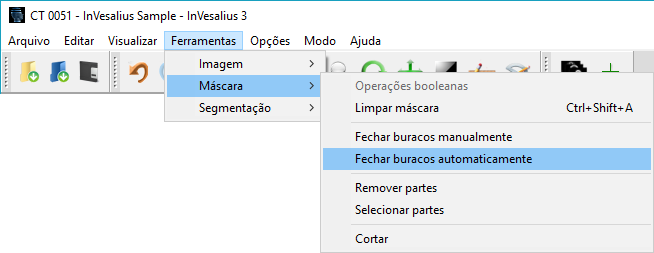
\includegraphics[scale=0.4]{menu_mask_automatic_fill_holes_pt.png}
\caption{Menu para acessar a ferramenta de fechamento de buracos automático.}
\label{fig:menu_mask_automatic_fill_holes}
\end{figure}

\begin{figure}[!htb]
\centering
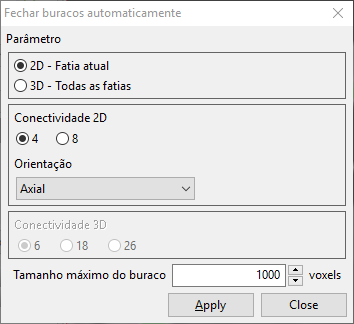
\includegraphics[scale=0.7]{mask_automatic_fill_holes_window_pt.png}
\caption{Tela para configurar parâmetros de fechamento de buracos.}
\label{fig:mask_automatic_fill_holes_window}
\end{figure}

Entre os parâmetros existe a opção de realizar o fechamento de buraco levando em consideração somente a fatia atual (\textbf{2D - Fatia Atual}) ou todas as fatias (\textbf{3D - Todas as fatias}) e suas respectivas conectividades, no caso 2D, conectividade $4$ ou $8$, conectividade $6$,$18$ ou $26$. No caso 2D é necessário indicar qual a janela será aplicado o fechamento de buracos, sendo axial, coronal ou sagital. No caso 3D se houver conectividade no buraco em diferentes fatias ele irá expandir para as demais fatias. 

Com os parâmetros configurados, clique no botão \textbf{Aplicar ou Apply}, caso o resultado não seja satisfatório, reconfigure o tamanho do buraco ou outros parâmetros como conectividade e aplique novamente. Para sair clique no botão \textbf{Sair ou Close}.

\section{Remover partes}

Antes de gerar a superfície é recomendável remover as partes desconexas não desejadas na máscara, dessa forma ao gerar a superfície será utilizada menores quantidades de memória RAM e o processo será mais rápido. Para remover as partes não desejáveis é necessário abrir a ferramenta de remover partes, clicando no menu \textbf{Ferramentas}, \textbf{Máscara} e \textbf{Remover Partes} (figura~\ref{fig:menu_mask_remove_part}). Em seguida irá ser exibido uma janela para configurar os parâmetros de seleção (figura~\ref{fig:mask_remove_parts_window}). É possível selecionar partes desconectas apenas na máscara 2D (\textbf{2D - Fatia atual}) ou em todo o conjunto de imagens, selecionando a opção \textbf{3D - Todas as fatias}. Também é possível selecionar suas respectivas conectividades, no caso 2D, conectividade $4$ ou $8$, conectividade $6$,$18$ ou $26$.

\begin{figure}[!htb]
\centering
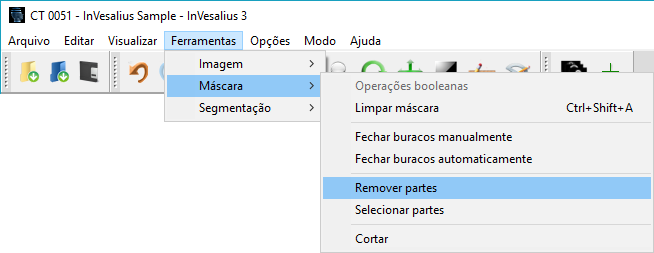
\includegraphics[scale=0.4]{menu_mask_remove_part_pt.png}
\caption{Menu para acessar a ferramenta de remoção de partes.}
\label{fig:menu_mask_remove_part}
\end{figure}

\begin{figure}[!htb]
\centering
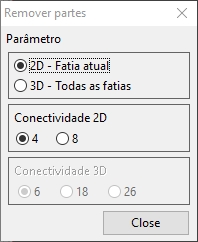
\includegraphics[scale=0.7]{mask_remove_parts_window.png}
\caption{Tela para configurar parâmetros de remoção de partes.}
\label{fig:mask_remove_parts_window}
\end{figure}

Selecionado os parâmetros desejados, basta clicar com o \textbf{botão direito do mouse} sobre a região que deseja remover. A figura~\ref{fig:mask_removed_part} apresenta uma exemplo de parte removida e não removida. Para sair da ferramenta clique no botão \textbf{Sair ou Close}.

\begin{figure}[!htb]
  \centering
  \subfloat[Imagem de entrada]{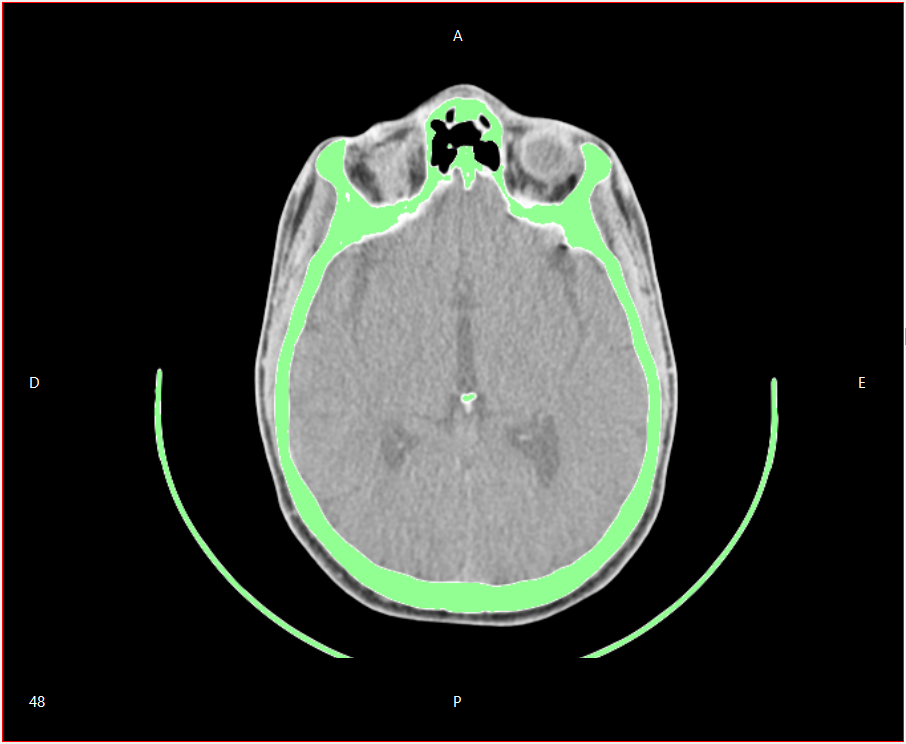
\includegraphics[width=0.45\textwidth]{mask_axial_complete.png}}  \qquad
  \subfloat[Imagem com suporte do tomografo removido]{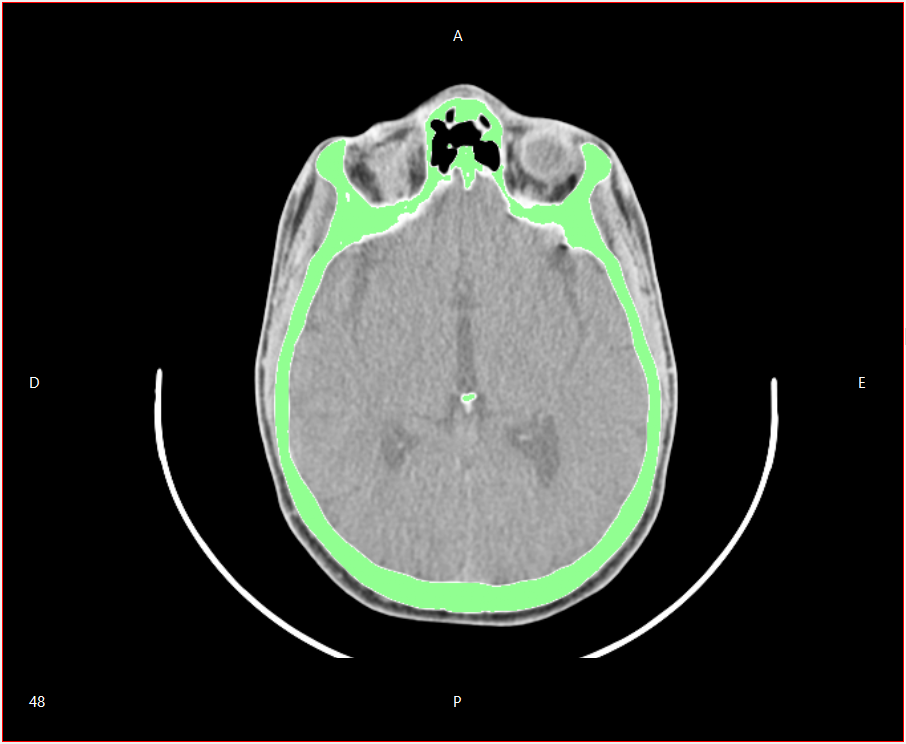
\includegraphics[width=0.45\textwidth]{mask_axial_selected_part.png}}
  \hfill
  \caption{Exemplo de região removida na máscara.}
  \label{fig:mask_removed_part}
\end{figure}

\section{Selecionar partes}

Para abrir a ferramenta de seleção de partes desconexas é necessário ir ao menu, \textbf{Ferramentas}, \textbf{Máscara} e por fim \textbf{Selecionar Partes} (figura~\ref{fig:menu_mask_select_part}). A ferramenta irá apresentar uma tela de configuração de parâmetros que consiste em qual conectividade será levada em consideração (figura~\ref{fig:mask_select_part}), podendo ser $6$, $18$ ou $26$ e o nome da nova máscara que irá ter a imagem resultante.

Todas as imagens a região que tem conectividade com o pixel selecionado. Para selecionar o pixel, é necessário clicar com o \textbf{botão esquerdo do mouse} em sobre o pixel desejado, o objeto irá ficar da cor vermelha, é possível selecionar vários objetos. Após a seleção é necessário clicar no \textbf{botão Ok}. A figura~\ref{fig:mask_selected_part}.a apresenta um objeto selecionado na cor vermelha e a figura~\ref{fig:mask_selected_part}.b  somente o objeto após ter fechado a ferramenta (\textbf{botão Ok}).

\begin{figure}[!htb]
\centering
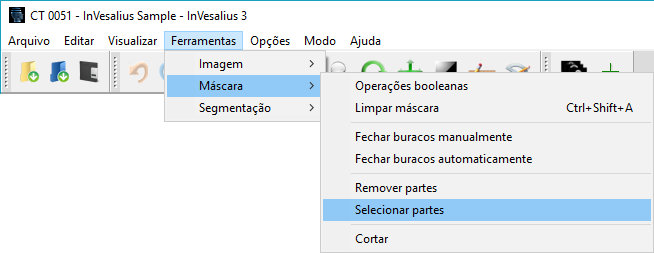
\includegraphics[scale=0.4]{menu_mask_select_part_pt.png}
\caption{Menu para acessar a ferramenta de seleção de partes.}
\label{fig:menu_mask_select_part}
\end{figure}

\begin{figure}[!htb]
\centering
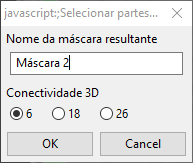
\includegraphics[scale=0.7]{mask_select_part_pt.png}
\caption{Tela para configurar parâmetros de seleção de partes.}
\label{fig:mask_select_part}
\end{figure}

\begin{figure}[!htb]
  \centering
  \subfloat[Região selecionada em vermelho]{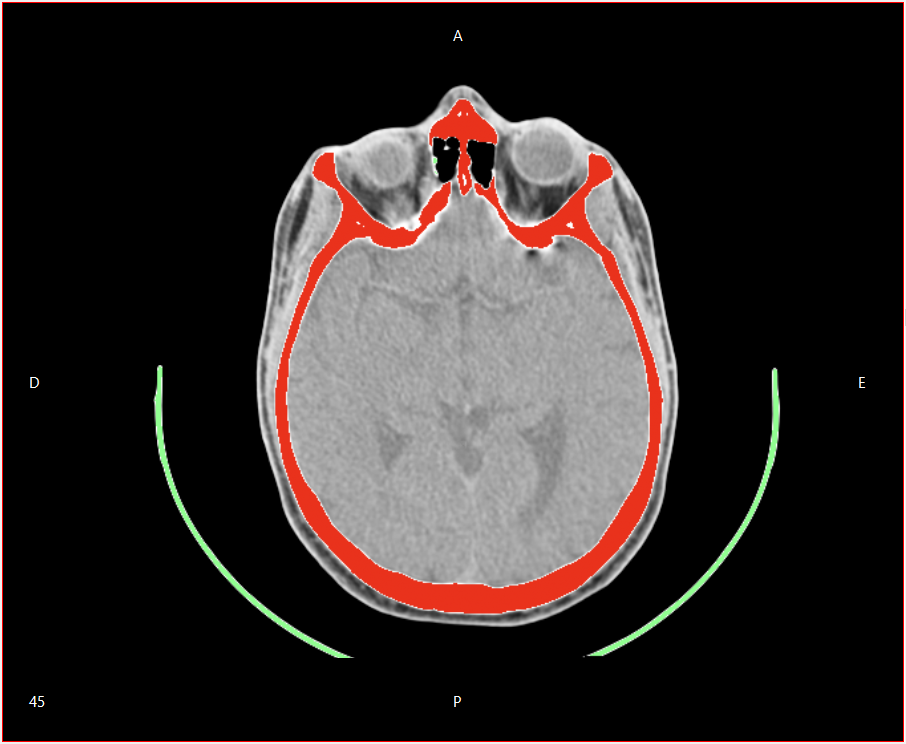
\includegraphics[width=0.45\textwidth]{mask_axial_select_part_pt.png}}  \qquad
  \subfloat[Imagem final, somente com a região selecionada]{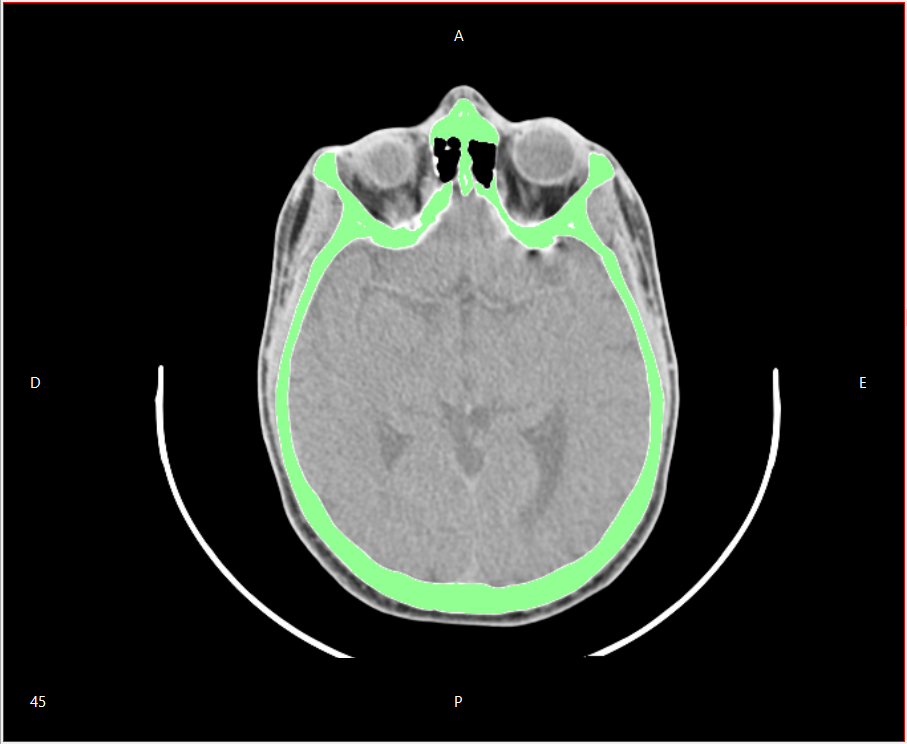
\includegraphics[width=0.45\textwidth]{mask_axial_selected_part_pt.png}}
  \hfill
  \caption{Exemplo de região selecionada na máscara.}
  \label{fig:mask_selected_part}
\end{figure}

\section{Cortar}

É possível cortar parte da máscara afim de selecionar uma região de interesse, isso pode ajudar reduzindo a quantidade de informações a ser processadas ao gerar superfície. Para abrir a ferramenta é necessário ir no menu \textbf{Ferramentas}, \textbf{Máscara} e por último \textbf{Cortar} (figura~\ref{fig:menu_mask_crop}).

\begin{figure}[!htb]
\centering
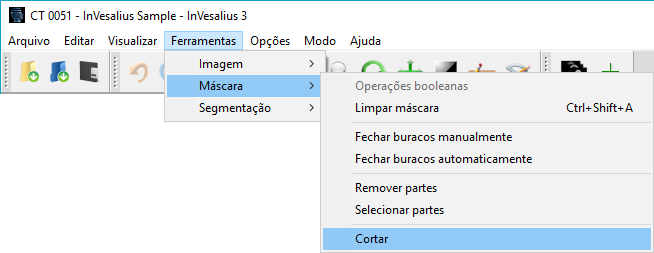
\includegraphics[scale=0.4]{menu_mask_crop_pt.png}
\caption{Menu para acessar a ferramenta de corte.}
\label{fig:menu_mask_crop}
\end{figure}

Será exibida uma caixa delimitadora em cada janela das orientações axial, coronal e sagital.